%\newpage
%\section{Initial design}%
%\label{sec:org68fdd80}
%
Following an analysis family tree of the products(remote controlled cars), the state of the art and the QFD matrix in fig.~\ref{fig:QFD}, an initial design of the product itself can be produced (fig.~\ref{fig:initial-design}).
The selected approach was top-down, in the sense that the requirements and specifications were addressed and that resulted in a general diagram of the product concept. Some macro-level decisions were made in this stage to narrow the solutions pool of the problems, as follows:
\begin{itemize}
\item  The car itself should be battery-powered, as it is a free-moving object that is intended to work in environments where trailing cables could interfere with its regular movement.
\item The device used to control the car should ideally be one already owned by the user, with an integrated screen (e.g.~smartphone), as it would make it more affordable and have a more straightforward interface.
\item The protocols for communication between the controlling device and the Rover should be chosen from within the pool of those readily available to smartphones (e.g. Wi-Fi, GPRS, Bluetooth) to keep the price of the overall product down and make it as practical as possible.
\item  The control and communication unit for the Rover should be divided into two modules: one which can measure and process sensor inputs and control the actuators in real-time, as well as communicate with the user-operated device through a low-latency connection. And another one which can interface directly with the camera module and manage data transmission to the user at the applicational level of the TCP/IP protocol stack, with enough throughput for the specified video resolution and frame rate. The latter should also exchange sensor reading values and commands with the user-controlled device, introducing redundancy to the controls and thus allowing for more reliable operation.
\end{itemize}

\begin{figure}[!ht]
\centering
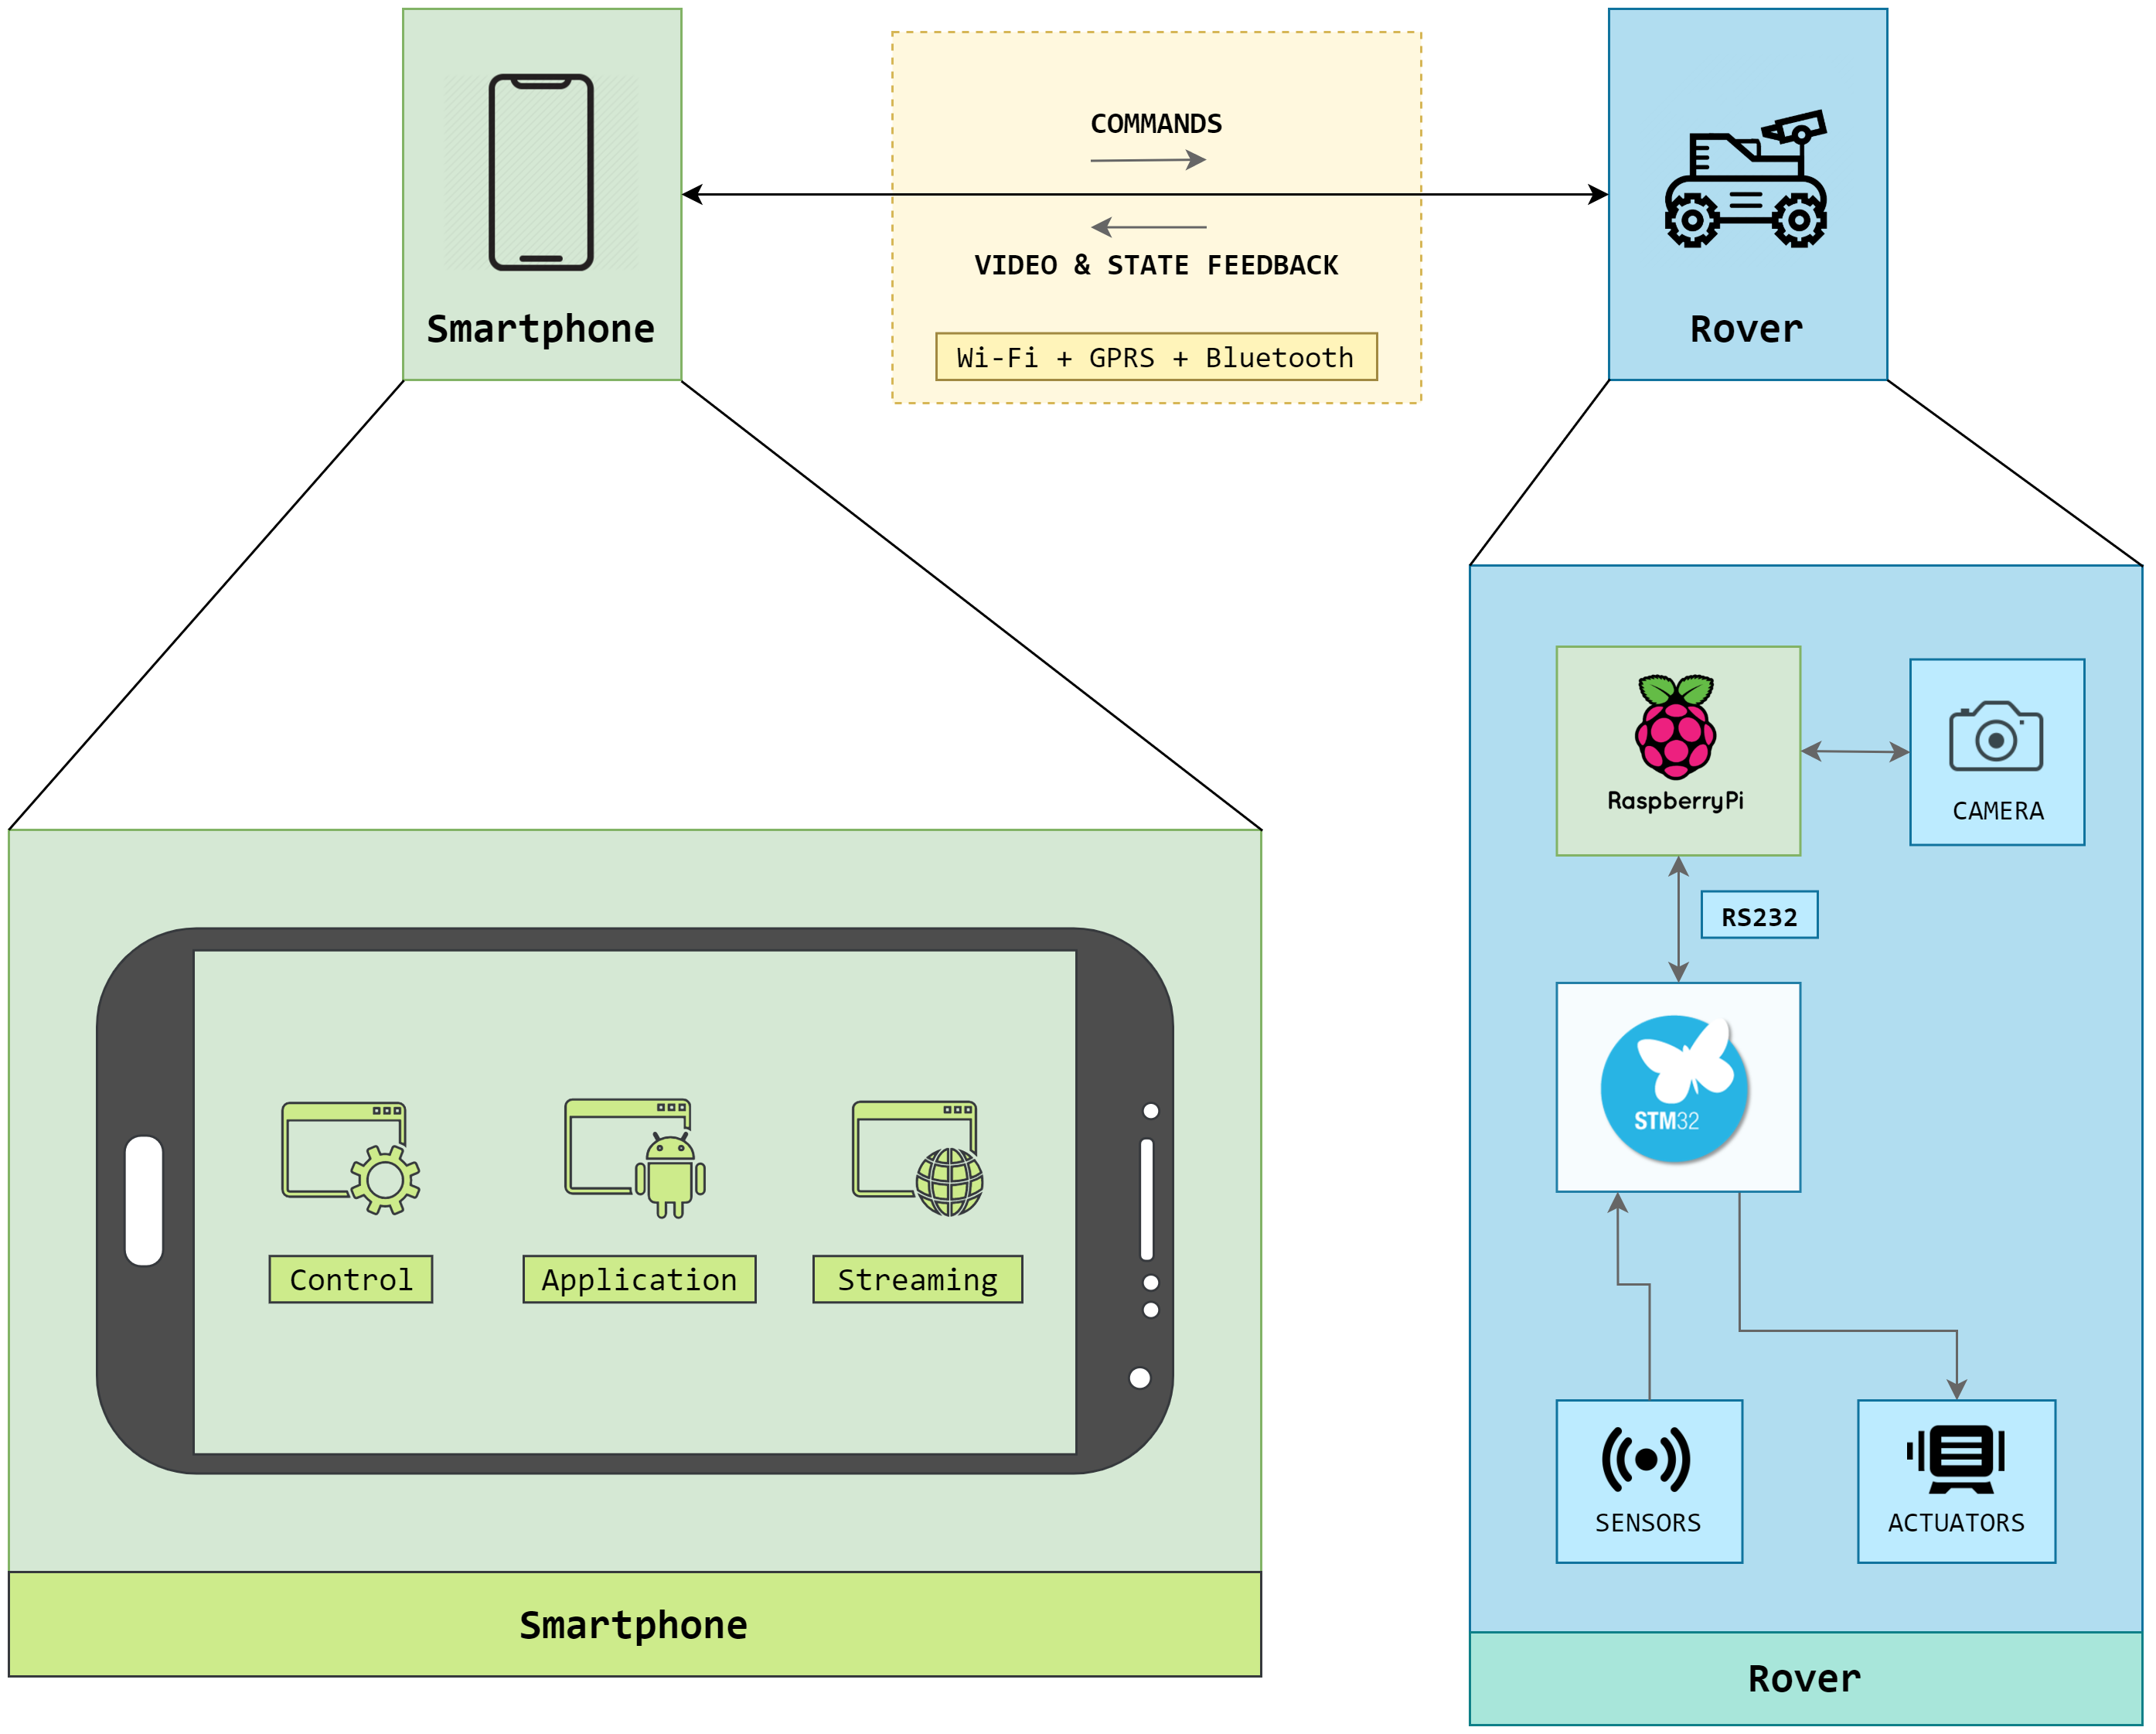
\includegraphics[width=0.9\textwidth]{./sec/img/initial_design_diagram.png}
\caption{\label{fig:initial-design}Initial design: Block diagram view}
\end{figure}

Thus, summarising, the initial design yields the system illustrated in
fig.~\ref{fig:initial-design}, comprised of:

\begin{itemize}
\item \textbf{ Raspberry Pi}: Interfaces with the camera directly, streaming that information to the smartphone. It also receives user commands and sends sensorial information it receives from the STM32 module back to the Smartphone, all through redundant Wi-Fi and GPRS connections;
\item \textbf{STM32}: Receives user commands and sends back sensorial information through a Bluetooth connection, information it also uses to control the actuators;
\item \textbf{Actuators}: DC Motors that control the movement of the Rover and headlights for nocturnal or low light conditions;
\item \textbf{Sensors}: Odometric sensors that support the detection of obstacles and luminosity sensors;
\item \textbf{Camera}: Device connected to the Raspberry Pi that allows the live stream of the car´s surrounding environment;
\item \textbf{Smartphone}: Grant visual feedback from the live feed of the camera also allowing the user to control the movement of the vehicle intuitively;
\end{itemize}

For simulation purposes and in conformance with the extraordinary conditions imposed by the recently enacted confinement measures, the need rose to create a virtual environment to simulate the various subsystems of the Rover. This solution allows for integrated testing without the need to deploy it to the hardware, as illustrated in fig.~\ref{fig:initial-design-2}.

The first of said subsystems is the Physical Environment Virtual Subsystem, which simulates the Rover and the physical environment, also receiving actuator inputs from the Navigation Virtual Subsystem, for which it generates the sensor readings. The latter also exchanges that information, as well as the status of the Rover and the commands from the user with the Smartphone module through a Bluetooth connection, which separates it from the non-simulated environment.

The Remote Vision Virtual Subsystem interfaces with the computer's Web Camera, which is meant to simulate the onboard camera of the Rover. Moreover, it can also communicate through Wi-Fi and GPRS, thus ensuring that communication is kept despite any failure from the Navigation Virtual Subsystem, as well as having shared access to the sensor reading values for monitoring of certain key parameters, depending on their refresh rate.

The RS232 connection between both controlling subsystems ensures proper synchronism and cooperation between them.
\newpage
%\clearpage
\begin{figure}[!ht]
\centering
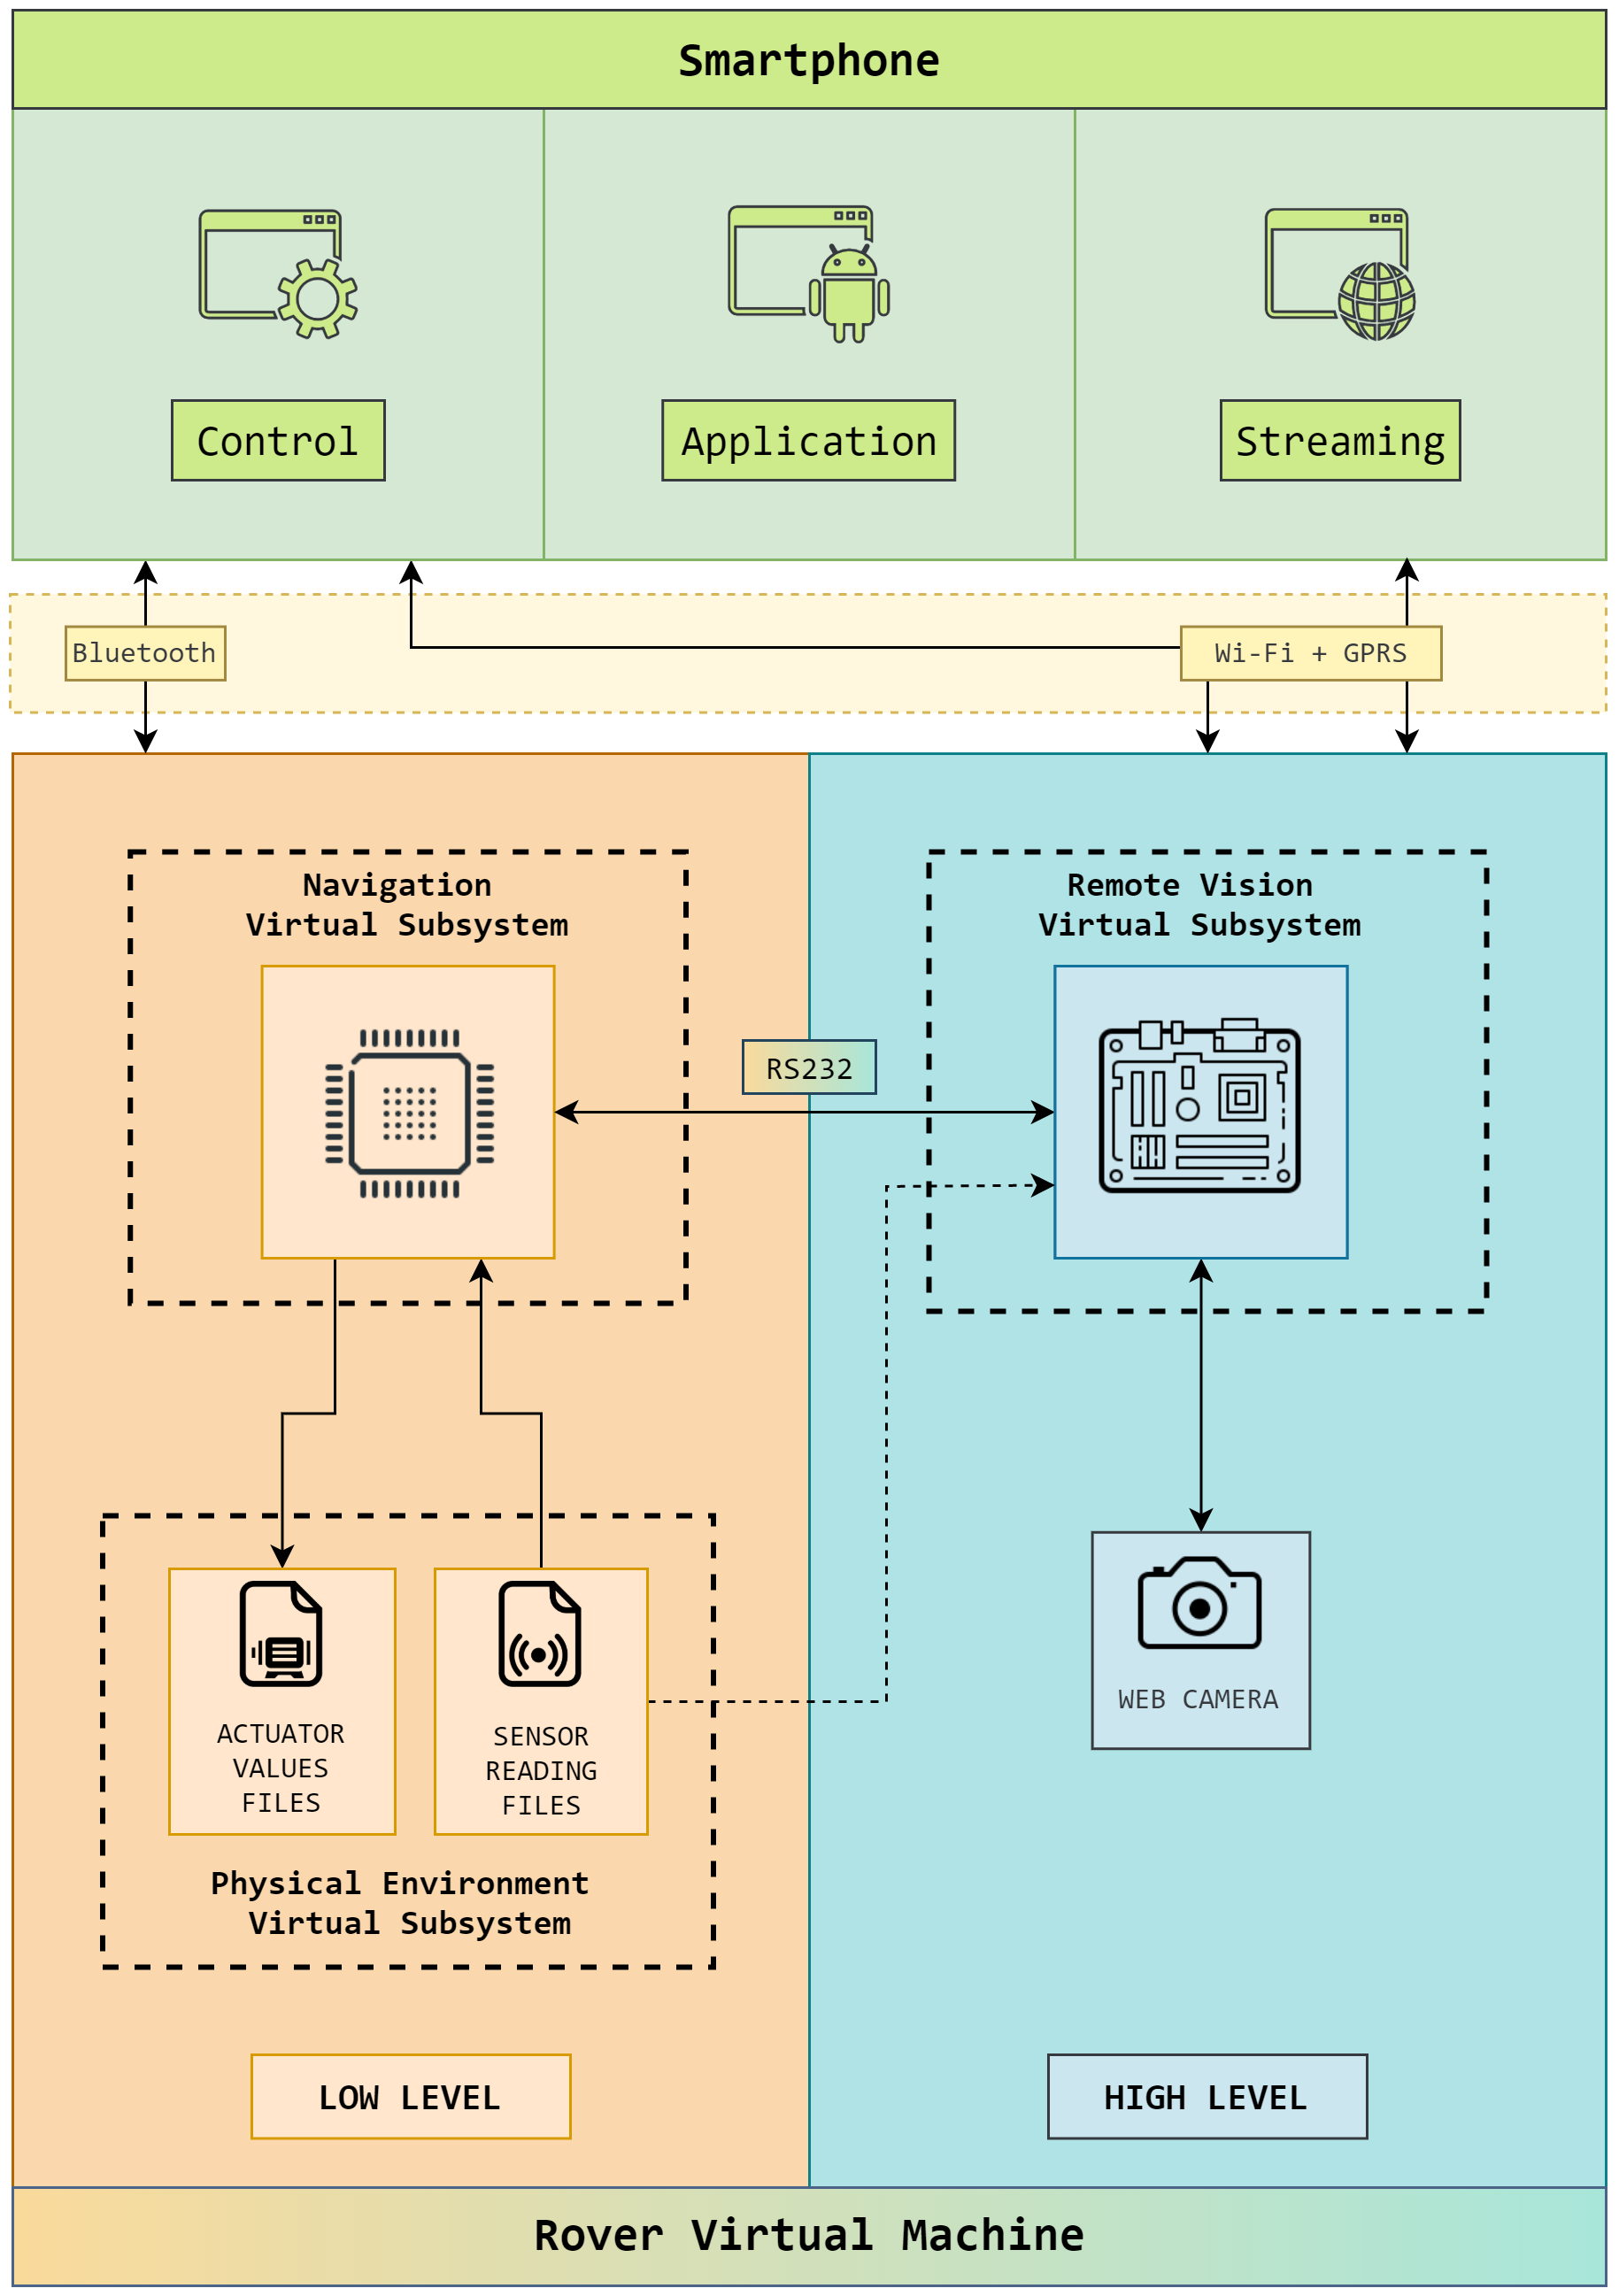
\includegraphics[width=0.6\textwidth]{./sec/img/initial_design_diagram_2.png}
\caption{\label{fig:initial-design-2}Initial design: Virtual environment block diagram view}
\end{figure}

%%% Local Variables:
%%% mode: latex
%%% TeX-master: "../Phase1"
%%% End: